\subsection{Interrelación Administrador Centro - Centro}

   \begin{description}
      \item[Definición] En esta interrelación se deja constancia de que pueden
      existir administradores de centro que administren los posibles centros
      que se establezcan en el sistema.

      \begin{itemize}
       \item Un \textit{Administrador Centro} puede administrar varios \textit{Centro}.
       \item Un \textit{Centro} puede ser administrado por varios
       \textit{Administrador Centro}.
      \end{itemize}

      \item[Características] La interrelación presenta las siguientes
                             características:

         \begin{itemize}
            \item \textbf{Nombre:} AC-C
            \item \textbf{Tipo de la interrelación:} Fuerte.
            \item \textbf{Cardinalidad de la interrelación:} N:M
                  \begin{itemize}
                     \item Administrador Centro: administra (0,n)
                     \item Centro: es\_administrado\_por (0,n)
                  \end{itemize}
            \item \textbf{Número de atributos:} Ninguno.
         \end{itemize}

      \item[Diagrama] La figura \ref{diagramaAC-C} muestra el diagrama de la
                      interrelación.
      \item \begin{figure}[!ht]
            \begin{center}
            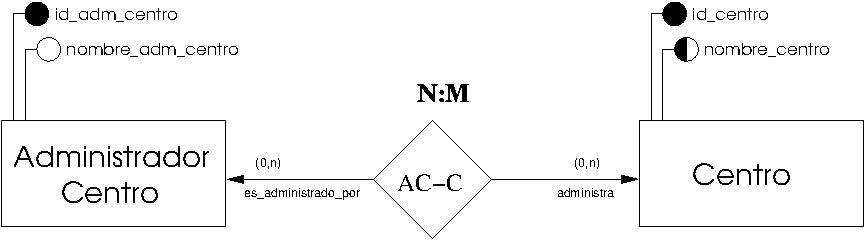
\includegraphics[]{07.Modelo_Entidad-Interrelacion/7.3.Analisis_Interrelaciones/diagramas/AC-C.pdf}
            \caption{Diagrama de la interrelación AC-C.}
            \label{diagramaAC-C}
            \end{center}
         \end{figure}

      \item[Ejemplo práctico del tipo de interrelación]

      \item \begin{center}
            \begin{tabular}{ | r r | }
            \hline
            \multicolumn{2}{ | c | }{\textbf{Tipo de interrelación AC-C}} \\
            \hline
            \textbf{Administrador Centro} & \\
            id\_adm\_centro & 9 \\
            \hline
            \textbf{Centro} & \\
            id\_centro & 15 \\
            \hline
            \end{tabular}
         \end{center}

   \end{description}
